% !TeX root = ./00.main.tex
\chapter{Proposta e metodologia}\label{cha:proposta}

\begin{resumocap}

  Este Capítulo apresenta a proposta deste trabalho e a metodologia elegida para
  atingir os objetivos.

\end{resumocap}

% Uma Implementação paralela do algoritmo de Detecção de Novidade em Streams MINAS 

A Internet das Coisas (\iot) é composta por milhares de dispositivos
conectados à Internet e distribuídos geograficamente.
Com capacidades diversas providas por elementos como sensores e atuadores, esses dispositivos produzem e
consomem Fluxos Contínuos de Dados (\streams) com diversos objetivos.
\nota{?}
Alguns cenários envolvem a mineração desses fluxos (\streamMining) em busca de
padrões para tomada de decisão e, por vezes requerem também baixa latência.
Para casos de baixa latência ou alta vazão, conexões adequadas para
processamento em nuvem nem sempre são possíveis ou desejáveis, para esses casos
computação em névoa (\fog) é uma solução.

\nota{?}
O tema de \streamMining envolve a classificação de novos elementos,
que podem tanto estar relacionados aos dados ou aos metadados das comunicações,
com base em
um modelo, porém como \streams variam temporalmente e são ilimitados, todas
classes contidas em um \stream não são previamente conhecidas.
A identificação e classificação de novas classes em \streams é denominada
Detecção de Novidades (\novelty, \nd) em \streams.
% \nota{?}
No tema de \nd, o surgimento e desaparecimento de classes é nomeado Evolução de Conceito
(\evolution) e a mudança no decorrer do \stream é denominado Mudança ou Deriva
de Conceito (\drift).

\nota{?}
Além dos aspectos inerentes a \streamMining, são considerados na construção de um
sistema que computa \streams a taxa de eventos (itens atômicos de um \stream)
gerados por cada produtor e o número de produtores nesse sistema, totalizando o
volume de eventos do sistema.
% Além do volume de eventos é necessário
Volumes elevados são dificilmente computados em apenas um nó (e muito menos em
um único núcleo processador) por esse motivo esses sistemas são distribuídos.

Sistemas que utilizam \nd para \streams gerados por dispositivos \iot devem
utilizar algoritmos que considerem os desafios inerentes de fluxos de dados
(\evolution e \drift) para adequada detecção de novidades e para tanto, requerem processamento em arquiteturas
que atendam os requisitos de volume de mensagens e latência de detecção.
O algoritmo MINAS é adequado para esse caso, pois trata os desafios de \streamMining porém não
tem ainda implementação que atenda os requisitos de volume e latência,
especialmente para aplicações \iot onde um ambiente de \fog é atrativo.

\newcommand{\flink}{\emph{Apache Flink}\xspace}
\newcommand{\mfog}{sistema M-FOG\xspace}

Para preencher a lacuna de algoritmo de \nd em ambiente \fog, propõem-se então
o \mfog, uma implementação do algoritmo MINAS sobre a plataforma \flink que
considera distribuição em um ambiente de \fog.

% \nota{Reestruturar:
%   A - remember,
%   B - cenário (iot, fog, stream),
%   C - problema (4.1, ND em fog, terminar com minas e cassales),
%   D - solução (4.2, apresetnação, resumo \mfog, metodologia)
% }
% \nota{Falta: fog, processamento distribuído de streams, detecção de novidade}

\section{Descrição da Implementação}\label{sec:descricao}

\newcommand{\source}{módulo auxiliar \emph{source}\xspace}
\newcommand{\sink}{módulo auxiliar \emph{sink}\xspace}

\newcommand{\offline}{módulo treinamento\xspace}
\newcommand{\classify}{módulo classificador\xspace}
\newcommand{\detector}{módulo detector\xspace}

Nesta Seção, apresenta-se o \mfog, objeto proposta deste trabalho.
O \mfog é composto de três módulos principais e dois auxiliares.
Os módulos principais implementam o algoritmo MINAS, sendo eles: \offline, \classify e \detector.
Dois módulos auxiliares são utilizados para correta avaliação:
\source (fonte) e \sink (sorvedouro, consumidor final).
Os módulos e as interações entre eles são ilustradas na \reffig{arch}.

A implementação proposta segue a arquitetura \idsiot formalizada por
\citeonline{Cassales2019a}, discutida na \refsec{cassales}.
A arquitetura \idsiot [e outras arquiteturas] estabelece que um serviço de
captura e tratamento de dados é instalado na borda de uma rede local com
dispositivos \iot.
Na presente implementação, esse serviço de captura e tratamento é representado
pelo \source.

O \source é dependente da fonte de dados, executando a transformação dos
formatos dos \datasets para um fluxo de dados compatível com o restante da
implementação.
Além de fornecer dados tratados para \mfog, o \source também fornece
dados para o \sink e \offline.

O \sink é responsável por agregar todos resultados do \mfog e,
juntamente com os valores do \dataset fornecidos pelo \source, por computar
as métricas de qualidade de classificação e métricas base para as métricas de
escalabilidade e métricas de recursos computacionais.

Os dados resultantes do serviço de captura e tratamento são ingeridos pela
aplicação no módulo \classify, por meio de conexão TCP (\emph{Transmission
Control Protocol}) fornecida pela plataforma \flink.
Na plataforma, com o modelo de classificação disponível, os exemplos são
classificados seguindo o algoritmo MINAS original discutido na \refsec{minas-og}.
A etiqueta atribuída pela classificação, ou meta-etiqueta de desconhecido,
juntamente com o exemplo original são enviados para o módulo \sink.
Além disso, se o exemplo não for classificado, o mesmo é enviado para o
\detector.

O \detector é responsável por executar o processo de detecção de
novidade, atualizando o modelo de classificação, e entrega do novo modelo
ao \classify.
Este também envia meta-informações sobre o processo de detecção de
novidade para o \sink.

% \nota{
% nao seria legal fazer um diagrama pq ai vc pode usar ate nos slides de como eh
% essa implementacao. Faz no draw io pra que de pra usar na monografia e de para
% enxergar na apresentacao
% }
\begin{figure}[!htb]
\centering
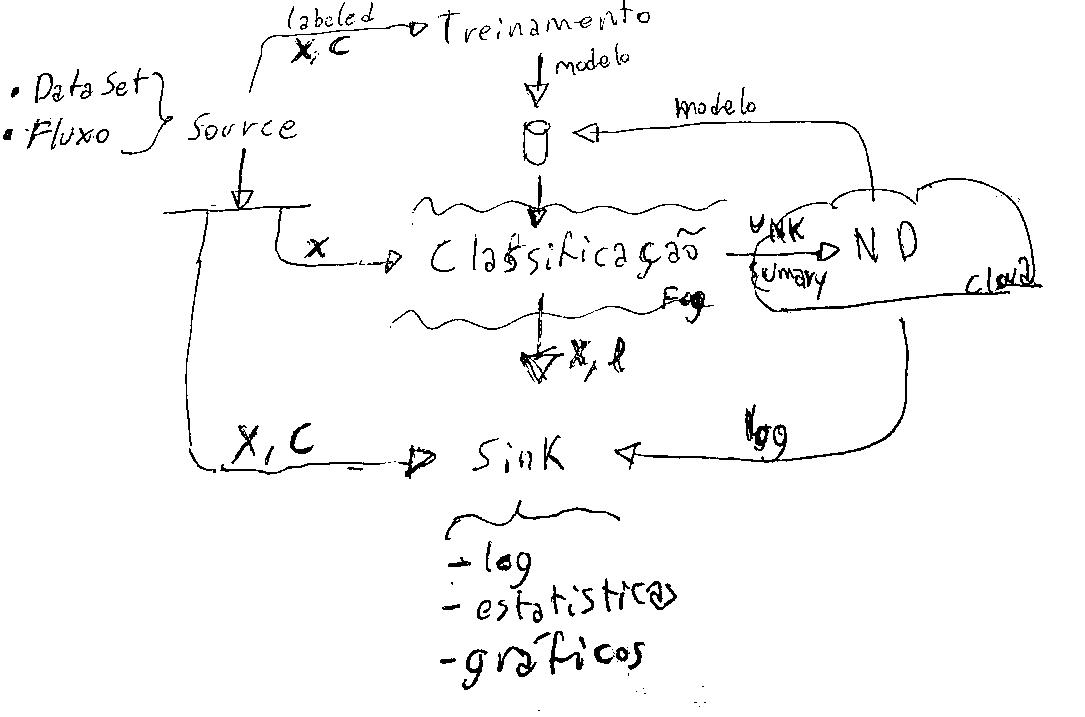
\includegraphics[width=\textwidth]{figuras/bwt_photo_arch.png}
\caption{Arquitetura \mfog.}
\label{fig:arch}
% \begin{tikzpicture}
% \end{tikzpicture}
\end{figure}

\nota{[Hélio] Como fica a distribuição do processamento?}

\section{Metodologia de Avaliação e Resultados Esperados}\label{sec:esperados}

% \nota{reestrutura 2:
%   A - cenario
%   B - metodologia (como, o que vai implementar [kafka, python, flink], como avaliar)
%   C - métricas (escalabilidade, qualidade)
%   D - resultados preliminares (python/kafka, flink)
% }

A avaliação da proposta apresentada será feita por meio de métricas extraídas da
literatura, divididas em duas partes: métricas de qualidade de classificação
e métricas de escalabilidade.

Métricas tradicionais de qualidade de classificação estabelecidas por trabalhos
de aprendizado de máquina não são adequadas para avaliar detecção de novidades em
\streams sem tratamento inicial. Felizmente, o tratamento necessário é
estabelecido por \citeonline{Faria2013} e expandido por
\citeonline{DaSilva2018,DaSilva2018thesis,Costa2019,Costa2019thesis}.
Além do tratamento estabelecido, as métricas tradicionais não são calculadas
somente para o conjunto completo, e sim para cada exemplo classificado; portanto,
as métricas têm como índice o instante $n$, informando a posição do exemplo em
relação ao fluxo.

O tratamento estabelecido das métricas de qualidade para \streamMining define
que as métricas são extraídas de uma matriz de erro de classificação
multi-classe $\mathbf{E}_n$ (\refequ{matrix}), adaptada para detecção de
novidade.
A matriz de erro é preenchida com o número de eventos da classe $c_i$ classificados com
etiqueta $l_j$ até o instante $n$.
A \refequ{classes} representa o conjunto de classes presentes nos eventos
do fluxo até o instante $n$ e a \refequ{labels} representa o conjunto
de etiquetas atribuídas pelo classificador a eventos até o mesmo instante.

\begin{align}
  % x_n &= classify_{n-1}(x_n)\\
  % e_{i, j} &= classify_{n-1}(x_n)\\
  \mathbf{C}_n &= \{ c_1, c_2, \cdots, c_M \}  \label{eq:classes} \\
  \mathbf{L}_n &= \{ l_1, l_2, \cdots, l_J \}  \label{eq:labels} \\
  \mathbf{E}_n &= \begin{pmatrix}
    e_{1,1} & e_{1,2} & \cdots & e_{1,J} \\
    e_{2,1} & e_{2,2} & \cdots & e_{2,J} \\
    \vdots  & \vdots  & \ddots & \vdots  \\
    e_{M,1} & e_{M,2} & \cdots & e_{M,J} 
  \end{pmatrix}  \label{eq:matrix}
\end{align}

As métricas de qualidade de classificação selecionadas para avaliar a
implementação \mfog são 
taxa de desconhecidos ($UnkR$ na \refequ{unkr}) \cite{Faria2013},
acurácia média ($acc$ na \refequ{acc})
e Macro F-score ($Fscore$ na \refequ{fscore}, também referido na literatura por
F1M) \cite{Sokolova2009,DaSilva2018thesis}.
As métricas são extraídas para todos os instantes $n$ da respectiva matriz de
erro $\mathbf{E}_n$.

\nota{'para todos os instantes n' ??}

\begin{align}
  \mathit{UnkR}       &= \frac{1}{M} \sum_{i=1}^{M} \frac{\#Unk_i}{\#ExC_i} \label{eq:unkr} \\
  \mathit{acc}        &= \frac{1}{M} \sum_{i=1}^{M} \frac{tp_i + tn_i}{tp_i+fn_i+fp_i+tn_i}
  = \frac{1}{M} \sum_{i=1}^{M} \frac{\#Acc_i}{\#ExC_i}  \label{eq:acc} \\
  \mathit{Precision}  &= \frac{1}{M} \sum_{i=1}^{M} \frac{tp_i}{tp_i+fp_i} \\
  \mathit{Recall}     &= \frac{1}{M} \sum_{i=1}^{M} \frac{tp_i}{tp_i+fn_i} \\
  \mathit{Fscore}_\beta &= (\beta^2 +1) \cdot
  \frac{
  \mathit{Precision} \cdot \mathit{Recall}
  }{
    \beta^2 \cdot \mathit{Precision} +\mathit{Recall}
  }\\
  \mathit{Fscore}_1   &= 2 \cdot \frac{
    \mathit{Precision} \cdot \mathit{Recall}
    }{
      \mathit{Precision} +\mathit{Recall}
    } \label{eq:fscore}
\end{align}
% = 2 \cdot \frac{tp}{2 \cdot tp + fn + fp}
% \mathcal{L}         &= \frac{-1}{N} \sum_{i=1}^{M} \sum_{j=1}^{J} y_{i,j} \log(p_{i,j})

% \nota{usar coeficiente d-intra vs d-extra grupo para determinar K de
% cada label. Também pode-se usar os mesmos coeficientes para _log_}

A transformação do fluxo de saída em uma matriz de erro é realizada no \sink
onde tem-se disponível o fluxo original com as etiquetas corretas e o fluxo
resultante da classificação.
Esse módulo deve levar em consideração que pode haver reclassificação de um
evento, previamente rotulado como desconhecido, em padrões oriundos de classe
novidade ou extensão devido ao processo de detecção de novidades executado
posteriormente ao surgimento do padrão em questão.

% Portanto os resultados são computados em função do fluxo de saída, então os $n$ nas
% equações são o índice do evento de saída.
% $\mathbf{unk}$ é o conjunto de eventos marcados como desconhecidos.
% \nota{oque eh unk? nesse paragrafo acima, erro de compilacao do latex?}

% \nota{frase confusa, eh so tirar o COMO e quebrar a frase: Esse módulo deve levar em consideração que
% COMO pode haver reclassificação de um evento, previamente rotulado como
% desconhecido, em padrões oriundos de classe novidade ou extensão devido ao
% processo de detecção de novidades executado posteriormente ao surgimento
% do padrão em questão}

% \begin{align}
%   E_{n,i,j} &= \bordermatrix{~ & c_i & \neg c_i \cr
%   l_j       & TP = \alpha           & FP = \gamma - \alpha                 \cr
%   \neg l_j  & FN = \beta - \alpha   & TN = n - (\alpha + \beta + \gamma)  \cr} \\
%   FM1       &= \frac{TP}{TP+\frac{FP+FN}{2}}
% \end{align}

% Os valores da matriz de erro para 

% \begin{align}
%   \alpha _j &= max( \{ |e_{i,j}|: i = 1 .. I \wedge \in \mathbf{E}_n \})
%           & \text{máximo da linha (etiqueta)} \\
%   a_j &= i: |e_{i,j}| = \alpha _j
%           & \text{índice da classe associada à etiqueta} \\
%   \beta   &= \sum_{j = 0}^{J} e_{i,j} : e_{i,j} \in \mathbf{E}_n
%           & \text{soma de uma coluna (etiqueta)} \\
%   \gamma  &= \sum_{i = 0}^{I} a_{i,j} : e_{i,j} \in \mathbf{E}_n
%           & \text{soma de uma linha (classe)}
% \end{align}

As métricas de escalabilidade selecionadas são: número de nós processadores,
tipo de processadores, uso de memória, tempo de processamento, taxa de eventos
processados e latência entre a produção e classificação de um evento.

% \begin{align}
%   \Delta { } t_n       &= t_{n,sink} - t_{n,source} \label{eq:delta-t} \\
%   \overline{\Delta { } t}_n       &= \frac{1}{N} \sum_{i=1}^{N} \Delta { } t_n  \label{eq:avg-delta-t} \\
%   \alpha &= \# processors \\
%   \gamma &= \frac{\overline{\Delta { } t}}{}
% \end{align}

% \nota{
% como assim os resultados sao validos so se tiverem essas metricas? Entao quer
% dizer que qual medida eh valida? Vc quis dizer que se as medicoes que vc extrair
% com essas metricas forem iguais as medicoes do minas original, entao ai eh
% valido. Eh Isso?
% }

% \nota{NAOOOOO!! Nao colocar frase depois do enumerate.
% Comeca um paragrafo novo ou continua ele com uma frase nova, nao pode fazer isso}

Da implementação \mfog é prevista execução de experimentos com \datasets
diversos, em especial os \datasets reais como \emph{Kyoto 2006+},
que contenham evolução de conceitos.
Os resultados desses experimentos contêm as seguintes métricas:

\begin{enumerate}[label={\alph*)}]
  \item Qualidade de classificação (taxa de desconhecidos, F1M);
  \item Escalabilidade (número de processadores, volume processado, tempo
  decorrido);
  \item Recursos computacionais utilizados (memória, tempo de processamento,
  operações de leitura e escrita).
\end{enumerate}

Para a validação da corretude da implementação com relação ao algoritmo MINAS
original, as métricas de qualidade de classificação serão extraídas com o mesmo
procedimento experimental previamente definido de ambos, \mfog e da
implementação original do algoritmo MINAS, e comparadas.

\subsection{Ambiente de Teste}

Para realização dos experimentos diversas configurações de ambientes são
propostas.
Os ambientes selecionados são local, nuvem e névoa.
As configurações consistem na distribuição de módulos da implementação \mfog
sendo executadas em combinações de ambientes nuvem e névoa com variada
quantidade de nós.

O ambiente local é composto por um único nó computacional, consistindo de um
computador pessoal equipado com um processador de 8 núcleos, $16GB$ de memória e
armazenamento em estado sólido (SSD) usado para o desenvolvimento e referência
em comparações.
O ambiente nuvem é provido pela utilização da infraestrutura de nuvem da
Universidade Federal de São Carlos (Cloud@UFSCar\footnote{Disponível em
\url{http://portalcloud.ufscar.br/servicos}}).
O ambiente de névoa (\fog) é composto por computadores de única placa
(\emph{Single Board Computer}) equipados com processador de arquitetura ARM de 4
núcleos, $1GB$ de memória, armazenamento em cartão SD (\emph{SD-card}) e
conectados por rede sem fio.

A combinação de diferentes distribuições tem por objetivo emergir padrões de
latência e qualidade que podem afetar implantações em ambientes reais que não
são geralmente destacados quando os experimentos são realizados em um único
nó ou ambiente.

Faz parte também do ambiente de teste os conjuntos de dados (\datasets)
\emph{KDD99} e \emph{Kyoto 2006+} que foram selecionados por motivos distintos.
O \dataset \emph{Kyoto 2006+} é foco desse trabalho pois contém dados ainda
representativos (até 2015) as característica desejáveis de um conjunto de dados
(realismo, validade, etiquetas previamente definidas, alta variabilidade,
reprodutibilidade e disponibilidade pública) são atendidas.
O \dataset \emph{KDD99} é amplamente utilizado em trabalhos de detecção de
anomalia e aqui é utilizado somente para que o leitor possa comparar com outros
trabalhos pois não possui mais a característica de realismo.

\section{Resultados preliminares}\label{sec:resultados}

No desenvolvimento parcial desta pesquisa, algumas experimentações e algumas
ferramentas de teste já forma desenvolvidas.
Alguns aspectos desses desenvolvimentos são descritos a seguir.
% obrigado hélio.

\newcommand{\kafka}{\emph{Apache Kafka}\xspace}
\newcommand{\python}{\emph{Python}\xspace}

\subsection{Implementação com \python e \kafka}

A primeira implementação e avaliação do \mfog realizada foi construída sobre a
linguagem \python com o sistema de fila de mensagens \kafka e a respectiva
biblioteca de conexão.
A escolha desse conjunto para a implementação deu-se devido à ampla
disponibilidade de bibliotecas de aprendizagem de máquina no ecossistema
\python e simplicidade geral da linguagem.
Na implementação desenvolvida, o sistema \kafka recebe mensagens e as armazena em tópicos distribuídos em
partições replicadas em nós de um \cluster, gerenciados por um nó mestre e
suportado pelo serviço de gerenciamento de configuração distribuída \emph{Apache
ZooKeeper}.
A aplicação \emph{Python} consome eventos através da interface \emph{Consumer API},
que expõe a distribuição através da associação de um consumidor às partições
mantidas pelo \kafka.

No entanto, a hipótese de que a distribuição de mensagens gerenciada pelo \kafka
se estenderia a processos consumidores, efetivamente distribuindo o volume de
mensagens entre eles igualmente, não se realizou nos experimentos realizados.
Os experimentos em questão foram compostos de 8 processos consumidores, um
processo produtor, uma instância \kafka com 8 partições em seu tópico principal
e uma instância \emph{Apache ZooKeeper} associada à instância \kafka.

% \nota{A hipótese era que o número de partições se igualaria ao número de 
% produtores e cada produtor associaria-se a uma partição.}

A hipótese era que, como o número de partições igualava o número de consumidores,
cada consumidor associaria-se a uma partição, distribuindo os dados igualmente
entre os consumidores para a paralelização a execução.
No entanto, essa hipótese foi refutada quando observou-se que o número de
mensagens consumidas por um dos 8 processos representava a maioria (mais de
80\%) do volume introduzido no sistema, o restante sendo distribuído entre
outros 3 processos e o restante dos processos não recebia nenhuma mensagem.
Portanto, a iniciativa de implementar o algoritmo MINAS em \python com \kafka e
atingir os objetivos de distribuição falhou, o que levou à reconsideração das
plataformas escolhidas.

\subsection{Implementação com \flink}

% \nota{citar ferramentas e a escolha só depois do python e kafka}
% \nota{entre flink e spark, outro grupo de pesquisa já está explorando spark}

A segunda alternativa explorada teve por inspiração o trabalho de
\citeonline{Viegas2019} e, como outro grupo de pesquisa já estava explorando
o algoritmo na plataforma \emph{Apache Spark}, a segunda implementação
foi baseada na plataforma \flink.

A plataforma flink tem modelos de processamento tanto de fluxos como em lotes.
O modelo em lotes é implementado como extensão do modelo de fluxos e, apesar
de não ser foco desse trabalho, mostrou-se útil para a construção do \offline,
já que o conjunto consumido por esse módulo é limitado.

Um desafio encontrado durante o desenvolvimento da implementação \mfog é a falta
de bibliotecas para a plataforma \flink, que disponibilizem versões adaptadas
à plataforma de algoritmos base para o algoritmo MINAS.
Em especial, a ausência dos algoritmos \emph{K-means} e \emph{CluStream} tem
atribuído carga não prevista sobre o processo de desenvolvimento.

% \nota{
% - offline, online, ND, Clustering \\
% - observação/Considerações de paralelização \\
% - Notas sobre implementação Python/Kafka/Minas (não escala como esperado) \\
% - Dificuldade no processamento distribuido em Flink. \\
% - complexidade bigO (?)
% }

% \chapter{Resultados Preliminares: implementação e testes}\label{cha:imp}
% cap 4: Implementação e testes
%     4.1. descrição da implementação
%         - offline, online, ND, Clustering
%         - observação de paralelização
%         - complexidade bigO (?)
%     4.2. cenário de teste 
%         - detecção de intrusão
%         - Arquitetura guilherme (dispositivos pequenos vs cloud)
%     4.3. Resultados de experimentos
%         - gráficos, tempos, tabelas...
%         - análises e comentários

% \begin{resumocap}
% \end{resumocap}

% \nota{Esse trabalho propos-se a fazer}

% % hélio
% notas sobre a distribuição do modelo
% - cenário com o processamento de novidades local
% - cenário com ND na nuvem

% - minas totalmente active

% helio amanha:
% a. Cenário, b. Problema, c. Proposta e d. Resultado Esperado.
% hermes:
% a. Monitoramento, classificação,
% b. detecção de novidades,
% c. executar em nós multi-core de maneira escalável,
% d. minas com mesma qualidade porém escalável.

% helio:
% Técnicas de firewall tradicional: allow all, deny all.
% Firewall moderno usa modelos.
% Minas como modelo.

% hermes
% iot, nós expostos vitima de ataque, novas funcionalidades ->
% firewall rigido vs modelos -> streams ->
% novidade -> minas -> big data -> discussão de localidade de dados
% paralelização

% motivação: testes preliminares do guilherme que fez teste com tais bases
% teve resultados promissores

% - implementar
% - paralelizar
% - avaliar
% - avaliar aprendizado local ou global trade-offs


% % luis
% O minas abre espaço 

% % hermes
% escalabilidade do algoritmo

% Kafka particiona e expoem esse particionamento ao consumidor.
% Tentei usar Python + Kafka, mas não escalou.

% Detalhar a implementação

% % hermes, esqueça kafka, foque em arquivos

% Realism: The network traffic used for building the dataset was obtained from real network traces. Moreover, MAWIFlow was built from over a year-long observation data of real network traces, enabling not only evaluation of the detection system during a specific period of time, but also the evaluation of its behavior over time, when facing new network traffic behavior;
% Validity: The network traces used for building the MAWIFlow dataset were collected from real network traces. Although MAWI (network traces used in MAWIFlow) is provided in a sanitized manner, i.e., payload is removed and sensitive data from network packet headers are encrypted, the network flow reconstruction is still possible. In this manner, the sanitization process used by MAWI does not affect the features’ values;
% Prior labeling: The event labels were identified by state-of-the- art unsupervised ML techniques (assessed by MAWILab). In this manner, supervised ML techniques can be evaluated regarding their performance as compared to unsupervised techniques;
% High Variability: MAWIFlow is highly variable not only owing to the used network traces but also owing to its long period of recording. The used network traces are real, valid, and collected from real network infrastructure, thereby it presents the expected variability from production environments. Nonetheless, owing to its long period of recording (the entire year 2016), the detection
% Reproducibility and Public Availability: The used network traces were collected from publicly available sources (MAWI). Moreover, BigFlow (Section 4) source code is also publicly available

% Para testar e demonstrar essa implementação um cenário de aplicação é construído
% onde seria vantajoso distribuir o processamento segundo o modelo \emph{fog}. Alguns
% cenários de exemplo são
% casos onde deve-se tomar ação caso uma classe ou anomalia seja detectada


% In time, process control and automation of industrial facilities, ranging from
% oil refineries to corn flakes factories \cite{Stonebraker2005}

% dataset kyoto não está disponível {http://www.takakura.com/Kyoto_data/}

% \nota{- detecção de intrusão\\
% - Arquitetura guilherme (dispositivos pequenos vs cloud)\\
% - Descrever a arquitetura IDS-IoT do paper do Guilherme \ cite{Cassales2019a}\\
% - dataset kyoto não está disponível\\
% - \ dataset kdd99\\
% - BigFlow com \ dataset atual e maior
% }

% % \subsection{Experimentos e Resultados}

% \nota{
% - gráficos, tempos, tabelas...\\
% - análises e comentários\\
% - Mostrar alguma implementação já feita e que esteja funcionando minimamente
% }

% \nota{Mostrar resultados mesmo que sejam bem simples e básicos,
% apenas para demonstrar que vc domina o ambiente e as ferramentas e
% que está apto a avançar no trabalho}

% \nota{discussão de 2020-02-01:\\
% passos feitos/a fazer\\
% 1. Entender Minas\\
% 2. Analisar/descrever data set KDD\\
% 3. Notas sobre implementação Python/Kafka/Minas (não escala como esperado)\\
% 4. BigFlow (data set mais novo, usa flink)\\
% 5. Plataforma Flink (processamento distribuído)\\
% Proposta\\
% 6. Implementar minas em Scala/Flink\\
% 7. Testar com data sets KDD e BigFlow\\
% 8. Validar/Comparar métricas com seus trabalhos correspondentes
% }

% \nota{lendo Quali Casssales:\\
% - Descrição do hardware utilizado pode conter:\\
%     - Arch, OS, Kernel,\\
%     - CPU (core, thread, freq),\\
%     - RAM (total/free size, freq),\\
%     - Disk (total/free size, seq RW, rand RW),\\
%     - Net IO between nodes (direct crossover, switched, wireless, to cloud) (bandwidth, latency).\\
% essas métricas permitem relacionar trade-offs para as questões de fog: Processar em node, edge ou cloud?
% }

% \nota{Provavelmente vou retirar o kafka da jogada em node/edge, deixando apenas em cloud.}
